\graphicspath{{\currfiledir/images/}}

\chapter{Metodologia}

%=====================================================

De um ponto de vista algorítmico e de estruturas de dados, os grafos têm alta representatividade de redes em geral, sejam estas representações de mapas, redes sociais ou até mesmo o fluxo de influências numa rede bibliográfica. Com isto, existem muitas e das mais diversas linhas de pesquisas sobre os grafos. Os estudos vão desde análise de uma rota otimizada em um mapa à análise do surto de uma transmissão viral. Seguindo-se nesta linha, o estudo sobre a análise da centralidade de caminhos mínimos é muito útil, pois infere quanto à sua importância/ relevância, além de representar diversos cenários da vida real. Um exemplo, dado um mapa, existem rotas que sempre são mais comumente usadas por transportes de carga rodoviário e afins, desta forma, espera-se que este trajeto demande de mais frequente manutenção. Este e muitos outros cenários nos levam a entender a importância do estudo e análise quanto a centralidade de caminhos mínimos.

O problema de centralidades em grafos é um problema muito explorado e já existem diversas técnicas para análise da centralidade de vértices, porém a centralidade de arestas, caminhos mínimos, presente neste mesmo escopo pesquisa, ainda carece de estudos. É um problema extremamente útil de se explorar, pois representa um enorme leque de aplicações da vida real.

Este trabalho é a parte conceitual e de aplicação direta do algoritmo e fluxo teórico proposto no trabalho da Alane de Lima da Universidade Federal do Paraná \cite{alane2021}. O problema da centralidade de caminhos mínimos é explorado no trabalho da Alane de um ponto de vista de aplicabilidade, pois o algoritmo e todo seu processo, já em teoria, são extremamente custosos em tempo de execução para grafos muito esparsos. A pesquisa dela busca métodos de análise da centralidade de caminhos mínimos de forma mais eficiente.

Dito isto, este trabalho irá mostrar a aplicação e fluxo de execução da proposta da proposta da Alane, mensurar a centralidade de caminhos mínimos. Os grafos que serão utilizados neste trabalho não são direcionados.

Para apresentação visual e conceitual da metodologia serão utilizados: um grafo simples, com 5 vértices; o modelo de grafo do clube de karatê de Zachary, que é uma rede social de um clube universitário de karatê \cite{zachary2009}; a rede de jogos de futebol americano entre as faculdades da Divisão IA durante a temporada regular do outono de 2000 \cite{networkxfootball2021}.

\section{Algoritmo}
Dados os grafos de entrada, a ideia geral do trabalho é obter todos os possíveis caminhos mínimos, isto é, executar o algoritmo de Dijkstra para cada um dos vértices do grafo. Como já mencionado, o algoritmo de Dijkstra, dado um vértice \emph{target}, constrói uma árvore de caminhos mínimos, sendo cada percurso da raiz até os nós da árvore, um caminho mínimo da raiz ao nó. Situações em que o grafo é conexo, a quantidade de caminhos mínimos de um vértice para todos os demais é de $n - 1$. Este processo será executado $n$ vezes, isto é, para todos os vértices do grafo.

O trabalho foi desenvolvido em \emph{Python 3} e para desenvolvimento central da aplicação foi usado a biblioteca \emph{NetworkX} \cite{networkx2021}.

A função \emph{main()}, serve de chamada central de outras subfunções que fazem o tratamento dos dados e que serão explicadas em sequência. De forma geral, esta função faz a construção de um grafo (\emph{linhas 2 - 4}), determina os caminhos mínimos para todos os vértices (\emph{linhas 5 - 8}), faz a computação de centralidade dos caminhos mínimos de um grafo (\emph{linha 7}) e exibe, na saída padrão, todos os caminhos mínimos com seus respectivos valores de centralidade (\emph{linha 8}).

\begin{lstlisting}[caption={Função central para chamada de subfunções.}]
	def main() -> None:
		G = simple_graph_generator()
		G = karate_club_graph_generator()
		G = football_graph_generator()

		dijkstraTrees = get_dijkstra_trees_from_a_graph(G)
		shortestPaths = get_shortest_paths(dijkstraTrees)
		all_shortest_paths_centrality(shortestPaths)
		print_all_paths_and_centrality(shortestPaths)
\end{lstlisting}

Para a geração de grafos de entrada, meu código possui 2 funções: o Algoritmo~\ref{sec4:funcao_simple_graph_generator}~(\mbox{\emph{simple~\textunderscore~graph~\textunderscore~generator()}}) e o Algoritmo~\ref{sec4:funcao_karate_club_graph_generator}~(\mbox{\emph{karate~\textunderscore~club~\textunderscore~graph~\textunderscore~generator()}}). Estas funções usam a biblioteca \emph{NetworkX} para construção manual de um grafo simples (Algoritmo~\ref{sec4:funcao_simple_graph_generator}) e o outro chama um grafo predefinido na própria biblioteca (Algoritmo~\ref{sec4:funcao_karate_club_graph_generator}). A Figura~\ref{sec4:representacao-simple-graph-generator} é uma representação visual do grafo gerado pela função \mbox{\emph{simple~\textunderscore~graph~\textunderscore~generator()}}.

\begin{figure}[!htb]
    \centering
	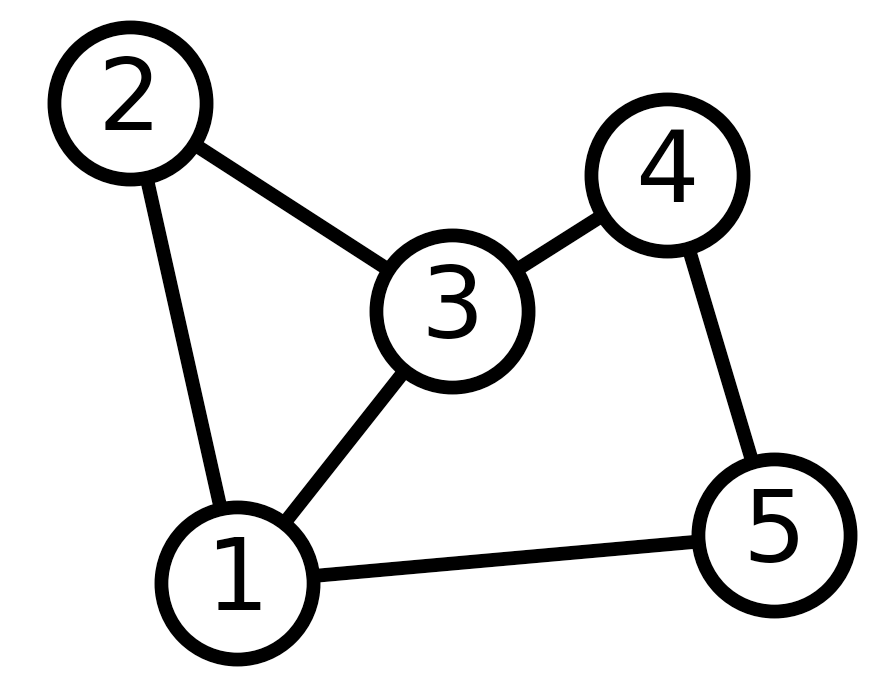
\includegraphics[scale=0.5]{representacao-simple-graph-generator.png}
    \caption{Grafo conexo e não direcionado de 5 vértices.}
    \label{sec4:representacao-simple-graph-generator}
\end{figure}

\begin{lstlisting}[caption={Função para gerar um grafo simples.}\label{sec4:funcao_simple_graph_generator}]
	def simple_graph_generator():
		G = nx.Graph()
		G.add_edge(1, 2)
		G.add_edge(1, 3)
		G.add_edge(1, 5)
		G.add_edge(2, 3)
		G.add_edge(3, 4)
		G.add_edge(4, 5)
		return(G)
\end{lstlisting}

\begin{lstlisting}[caption={Função para gerar o modelo de grafo do clube de karatê de Zachary.}\label{sec4:funcao_karate_club_graph_generator}]
	def karate_club_graph_generator():
		G = nx.karate_club_graph()
		for v in G:
			print(f"{v:4} {G.degree(v):6}")
		return(G)
\end{lstlisting}

Tendo os grafos de entrada criados, agora iniciaremos o processo de tratamento destes dados.

Dado um grafo de entrada, o Algoritmo~\ref{sec4:funcao_get_dijkstra_trees_from_a_graph} (\mbox{\emph{get~\textunderscore~dijkstra~\textunderscore~trees~\textunderscore~from~\textunderscore~a~\textunderscore~graph()}}) trata os dados de entrada para passar por cada um dos vértices, gerando a árvore de Dijkstra. Estes dados são armazenados em um dicionário de caminhos mínimos, indexado pelos rótulos dos vértices.

\begin{lstlisting}[caption={Função para tratar os dados de um grafo de entrada e gerar um dicionário de árvores de Dijkstra, indexado pelos rótulos dos vértices do grafo.}\label{sec4:funcao_get_dijkstra_trees_from_a_graph}]
	def get_dijkstra_trees_from_a_graph(g: dict) -> dict:
		graphDict = {}
		for node in g:
			if node not in graphDict:
				graphDict[node] = single_source_dijkstra(g, node)[1]
		return graphDict
\end{lstlisting}

No próximo passo, o Algoritmo~\ref{sec4:get_shortest_paths_from_dijkstra_trees} (\mbox{\emph{get~\textunderscore~shortest~\textunderscore~paths~\textunderscore~from~\textunderscore~dijkstra~\textunderscore~trees()}}) é uma etapa de refinamento dos dados previamente obtidos, isto é, ele pega os dados do dicionário de caminhos mínimos (\mbox{\emph{get~\textunderscore~dijkstra~\textunderscore~trees~\textunderscore~from~\textunderscore~a~\textunderscore~graph()}}) e faz algumas operações, como retirada de colchetes nos nomes dos caminhos mínimos e afins.

\begin{lstlisting}[caption={Função para refinamento do dicionário de caminhos mínimos.}\label{sec4:get_shortest_paths_from_dijkstra_trees}]
	def get_shortest_paths_from_dijkstra_trees(graphDict: dict) -> dict:
		pathDict = {}

		for i in graphDict.values():
			for j in i.values():
				path = str(j).replace("[", "").replace("]", "")
				if path not in pathDict and len(path) > 1:
					newPathInfo = PathInfo(0, len(j))
					pathDict[path] = newPathInfo

		return pathDict
\end{lstlisting}

Agora sim, tendo-se os dados refinados, esta etapa visa calcular a centralidades dos caminhos mínimos, Algoritmo~\ref{sec4:all_shortest_paths_centrality} (\mbox{\emph{all~\textunderscore~shortest~\textunderscore~paths~\textunderscore~centrality()}}). A centralidades dos caminhos mínimos do grafo é calculada da seguinte forma: para cada caminho mínimo $cm_1$, verifique em todos os demais caminhos mínimos se $cm_1$ está presente como subcaminho mínimo (\emph{linhas 2 - 5}); em caso positivo, contabilize $+1$ na centralidade de $cm_1$ (\emph{linha 6}); estas etapas são repetidas para todos os demais caminhos mínimos (\emph{linhas 2 - 6}); feito isto, agora a última etapa é referente a normalização dos valores (\emph{linhas 11 - 13}), pois é comumente visto a ponderação de valores com numerações entre $0$ e $1$, ou seja, quanto mais próximo de 1, maior a centralidade do caminho mínimo.

\begin{lstlisting}[caption={Função para cálculo da centralidade dos caminhos mínimos.}\label{sec4:all_shortest_paths_centrality}]
def all_shortest_paths_centrality(pathDict: dict) -> dict:
	# Check if i is contained in j. If it is, plus one
	for i in pathDict:
		for j in pathDict:
			if i in j:
				pathDict[i].centrality += 1

	# Get the number of Dijkstra trees
	numTrees = len(pathDict)

	# Normalizing centrality values
	for path in pathDict:
		pathDict[path].centrality /= numTrees * pathDict[path].numNodes
\end{lstlisting}

%=====================================================
